%\documentclass[12pt,a4paper,twoside,openright,fleqn]{memoir}
\documentclass[10pt]{article}
\usepackage[danish]{babel}
\usepackage[ansinew]{inputenc}
\usepackage{graphicx}
\usepackage{subfig}
\usepackage{listings}
\usepackage{natbib}
\usepackage{titleref}

\begin{document} 

%\newcommand{\oversaet}[1]{(\textit{#1})}


\title{Master Thesis}
\author{Thomas Thyregod 20051688\\ Morten Daugaard 20051715\\ \texttt{ tysse, taghof }@cs.au.dk\\\\ Department of Computer Science, University of Aarhus\\ Aabogade 34, 8200 Aarhus N, Denmark\\\\
\hline\\
\vspace{4cm}\\
\makeatletter
\texttt{Semi Autonomous Navigation}\\
\texttt{for Arial Robots}\\
\vspace{4cm}\\
\hline\\
}
\date{\today}
\maketitle
\newpage

\pagestyle{headings}

\section*{Resume Abstrakt}

\pagebreak

\tableofcontents

\pagebreak

\section{Introduktion}
\subsection{omr�det, teknologi}
\subsection{}
\subsection{}

\pagebreak
\section{AR.Drone}
AR.Drone er en quadrocopter fremstillet og udviklet af det franske
firma Parrot. En quadrocopter benytter fire faste rotorer til at
generere opdrift, samt til at styre sin bev�gelse i rummet. 
\\AR.Drone blev introduceret i 2010 og har siden fundet stor anvendelse, ikke
blot som et stykke avanceret leget�j, men ogs� som en
udviklingsplatform til forskere og studerende. En AR.Drone kommer med et
s�t sensorer best�ende af to kameraer(et vertikalt nedadrettet og et
horisontalt fremadrettet), en h�jdem�ler, gyroskop(til at m�le
h�ldning, kr�ngning og drejning), samt et accelerometer. I 2012 ventes
en opdateret udgave af AR.Drone, denne forventes at tilf�je HD kamera,
trykm�ler og kompas til platformen.
\\AR.Drone er opbygget som en letv�gtskonstruktion af kulfiber, plast og
skummateriale og kommer med to forskellige skumskjold til henholdsvis
indend�rs og udend�rs flyvning.

\begin{figure}[h]
\centering
  \subfloat[Indend�rsskjold]{
    \label{fig:indend�rsskjold}
    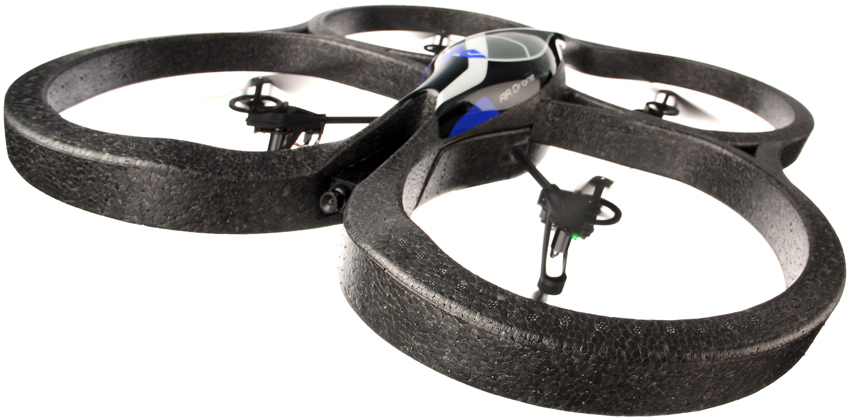
\includegraphics[width=0.45\textwidth]{parrot-ardrone.jpg}
  }
  ~ %add desired spacing between images, e. g. ~, \quad, \qquad etc. (or a blank line to force the subfig onto a new line)
  \subfloat[Udend�rsskjold]{
    \label{fig:udend�rsskjold}
    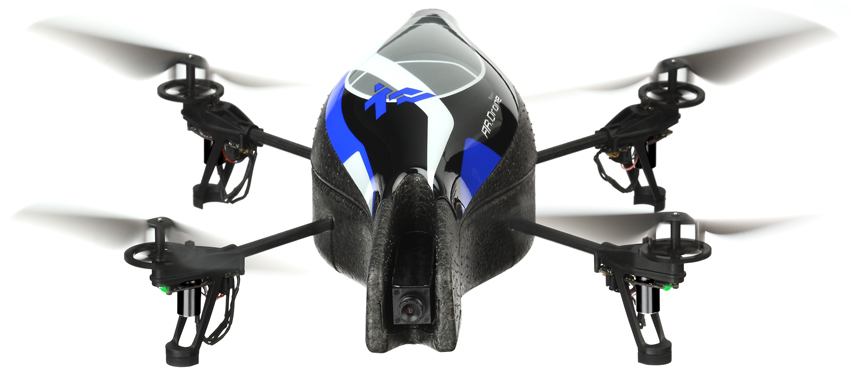
\includegraphics[width=0.45\textwidth]{parrot-ardrone-outdoor.jpg}
  }
  \caption{AR.Drone med indend�rs- og udend�rsskjold}
  \label{fig:ardrone}
\end{figure}
 
\subsection{Hardware}
Som de fleste robotter best�r AR.Drone af et antal sensorer, et antal
aktuatorer og en styringsenhed. 
\\AR.Drone er udstyret med to kameraer, det fremadrettede er en 93
graders CMOS sensor som kan levere 640x480 billeder(selvom
resourceknaphed g�r at opl�sningen der transmitteres fra dronen
kun er 320x240(QVGA)) med en framerate p� 15/s. Det nedadvendte kamera er
en 64 graders CMOS sensor, der tager billeder i 176x144(QCIF) med en
framerate p� 60/s.
\\Til at bestemme dronens h�jde over jorden anvendes en ultrasonisk
h�jdem�ler, denne opererer ved at udsende en ultralydspuls og herefter
m�le tidsintervallet der g�r f�r ekkoet m�les. H�jdem�leren er angivet
til at virke op til seks meters h�jde og er rent fysisk placeret p�
dronens navboard. Det er v�rd at bem�rke, at h�jdem�leren ikke m�ler
h�jden p� et specifikt punkt, men derimod returnerer den mindste h�jde
i et omr�de som det p� (fig).

gyroskoper

accelerometer

embedded computer

motorer
  
\subsection{Software}
%\lstinputlisting[language=Python]{../drone.py}
\subsection{Kommunikation}

\subsection{Fysik}

\pagebreak

\appendix

\bibliographystyle{abbrv}
\bibliography{referencer}

\section{Appendix header A}



\end{document}

%\begin{center}
%  \includegraphics[scale=0.35]{pic/selfserv.jpg}
%\newline
%\textbf{Figur 1}
%\end{center}
